\chapter{Tracking significance calculation}
\label{APP::LIANDMA}

For data analyzed using the standard \Trk\ analysis
(section~\ref{SEC::ANALYSIS::TRACKING}), a number of different
measures of ``significance'' can be
defined. \citet{REF::LIANDMA::1983APJ} discuss the derivation and
merits of three such measures, reproduced below as
eqns.~\ref{EQN::APPLIANDMA::5}, \ref{EQN::APPLIANDMA::9} and
\ref{EQN::APPLIANDMA::17}, corresponding to eqns. 5, 9 and 17
respectively in the original paper. As discussed in the paper, the
simple propagation of errors calculation, $S_5$, is not distributed as
Gaussian n the absence of a source, particularly when $\rho\ll1$ or
$\rho\gg1$.  It systematically underestimates the true significance of
a detection. An improved model of the background gives, $S_9$, which
is shown to overestimate the significance. Taking the ratio of the
likelihood of the source being present to the null hypothesis being
true (no source present) gives $S_{17}$, which is shown to be
distributed as Gaussian.
\begin{eqnarray}
S_5 & = & \frac{N_\mathrm{On}-\rho N_\mathrm{Off}}{\sqrt{N_\mathrm{On}+\rho^2N_\mathrm{Off}}}\label{EQN::APPLIANDMA::5}\\
S_9 & = & \frac{N_\mathrm{On}-\rho N_\mathrm{Off}}{\sqrt{\rho(N_\mathrm{On}+N_\mathrm{Off})}}\label{EQN::APPLIANDMA::9}\\
S_{17} & = & \sqrt{2}\left\{N_\mathrm{On}\ln\left[\frac{1+\rho}{\rho}\left(\frac{N_\mathrm{On}}{N_\mathrm{On}+N_\mathrm{Off}}\right)\right]\nonumber\right.\\
&  & + \left.N_\mathrm{Off}\ln\left[(1+\rho)\left(\frac{N_\mathrm{Off}}{N_\mathrm{On}+N_\mathrm{Off}}\right)\right]\right\}^{1/2}\label{EQN::APPLIANDMA::17}\\
S_{\Delta\rho} & = & \frac{N_\mathrm{On}-\rho N_\mathrm{Off}}{\sqrt{N_\mathrm{On}+\rho^2N_\mathrm{Off}+\Delta\rho^2N_\mathrm{Off}^2}}\label{EQN::APPLIANDMA::DELTARHO}
\end{eqnarray}

No attempt was made by \citet{REF::LIANDMA::1983APJ} to account for an
error in the \On/\Off\ ratio, $\rho$. They concentrated on classes of
experiments in which $\rho$ arose due to differences in the on-source
and off-source observing times, which would be known to high
accuracy. For the \Trk\ analysis, there is a statistical error on the
value of $\rho$ arising from the fact that it must be calculated from
dark-field data, with $N^*_\mathrm{On}$ counts with $\alpha<15^\circ$
and $N^*_\mathrm{Off}$ counts with $20^\circ<\alpha<65^\circ$:
\[\rho = \frac{N^*_\mathrm{On}}{N^*_\mathrm{Off}}\pm
\frac{N^*_\mathrm{On}}{N^*_\mathrm{Off}}\sqrt{\frac{1}{N^*_\mathrm{On}}+\frac{1}{N^*_\mathrm{Off}}}\]
Propagation of errors, including $\Delta\rho$, leads to
$S_{\Delta\rho}$ (eqn.~\ref{EQN::APPLIANDMA::DELTARHO}), which becomes
equal to $S_5$ as $\Delta\rho\rightarrow0$.

Following \citet{REF::LIANDMA::1983APJ}, a simple Monte Carlo (MC)
simulation was perfomed to test the four ``significance
measures''. Random values for of $N_\mathrm{On}$ and $N_\mathrm{Off}$ 
was generated from Poisson distribution with appropriate 
$\langle N_\mathrm{On}\rangle$ and $\langle N_\mathrm{Off}\rangle$.  
It was assumed that there is a true value
for the tracking ratio, $\rho^T=1/3$ which connects the
distributions of \On\ and \Off\ counts, i.e. that $\langle
N_\mathrm{On}\rangle=\rho^T\langle N_\mathrm{Off}\rangle$. To match
the simulation with the exposures used in this study, a value of
$\langle N_{\Off}\rangle\approx6300\,\mathrm{counts}$ was used,
typical for a ten hour exposure. To calculate of the significances, a
random, ``measured'', value for the tracking ratio, $\rho^M$, was
generated, distributed around $\rho^T$ with $\Delta\rho^M=0.0015$. The
size of $\Delta\rho$ was taken from a calculation of the tracking
ratio with real data in 2000/2001 \citep{REF::HORAN::2001THESIS}.

Figure~\ref{FIG::APPLIANDMA::SIGMA} shows the frequency of
``$>x\sigma$'' results with each of the significance measures. In the
case of $\Delta\rho=0$, \citet{REF::LIANDMA::1983APJ} show, from MC,
that $S_{17}$ is normally distributed. With $\Delta\rho\neq0$, this
conclusion is no longer valid, as is expected, since no consideration
to $\Delta\rho$ given in its calculation. It can be seen that the
measure which comes closest to a Gaussian distribution is $S_5$, at
least with the values for $\rho^T$, $\Delta\rho$ and $\langle
N_{\Off}\rangle$ used in the simulation. This is attributed to a
cancellation of the effect of systematic under-estimation the absence
of $\Delta\rho$ (seen by \citet{REF::LIANDMA::1983APJ}) with the
overestimation due to $\Delta\rho\neq 0$. It is expected that, as
$\Delta\rho$ increases, $S_{\Delta\rho}$ would become the only
significance measure, of the four listed above, representative of a
Gaussian distribution.

\begin{figure}[ht]
\centerline{\resizebox*{\textwidth}{!}{\rotatebox{270}{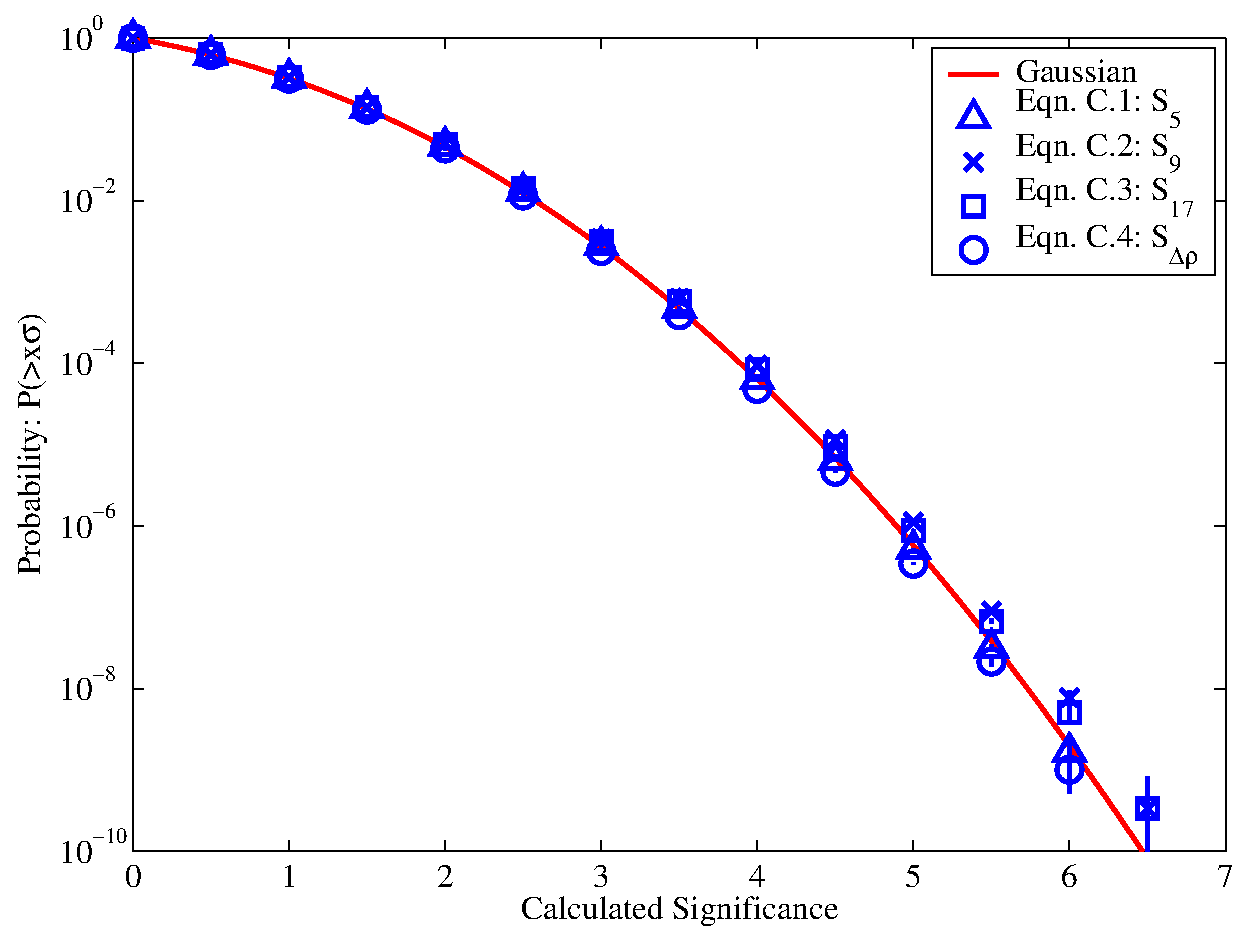
\includegraphics[draft=false]{plots/app-liandma/liandma.pdf}}}}
\caption{\label{FIG::APPLIANDMA::SIGMA} Monte Carlo evaluation of 
frequency of $>x\sigma$ results with different ``significance
measures''. Only positive excesses are considered in the simulation,
so $P(>0\sigma)=1$.}
\end{figure}
